\documentclass[11pt,a4paper]{article}

\usepackage[margin=2.3cm]{geometry}
\usepackage[T1]{fontenc}
\usepackage{lmodern}
\usepackage{microtype}
\usepackage{graphicx}
\usepackage{booktabs}
\usepackage{tikz}
\usetikzlibrary{positioning,arrows.meta,fit}
\usepackage[hidelinks]{hyperref}
\usepackage{caption}

\setlength{\parskip}{4pt}
\setlength{\parindent}{0pt}
\newcommand{\file}[1]{\texttt{#1}}
\emergencystretch=2.5em
\tolerance=2000

\title{\textbf{LANBoard: a LAN collaborative whiteboard}\\[4pt]
\large Team contributions and explanation report}
\author{Computer Networks Lab Project 2026\\
Indian Institute of Information Technology, Design and Manufacturing\\
(IIITDM) Kancheepuram}
\date{15 November 2026}

\begin{document}
\maketitle

\begin{center}
\begin{tabular}{llll}
\toprule
\textbf{Name} & \textbf{Roll no.} & \textbf{Area} \\
\midrule
Yashvanth S & CS24I1029 & Server core and state, integration, tests, docs \\
Jeevanandham T & CS24I1035 & Protocol and networking \\
Akula Sai Teja & CS24I1054 & Canvas and drawing, builds and CI \\
Nithillakrishi P Y & CS24I1039 & User interface and collaboration \\
\bottomrule
\end{tabular}
\end{center}

\section{What LANBoard is}

LANBoard is a shared whiteboard that works only on a local network. One machine runs the
server. Everyone else opens the client, finds the server in a ``Nearby servers'' list and joins a
room with a short code. After that, all of them can draw, write text, add sticky notes and images,
annotate PDF slides and chat, and every change shows up on the other screens almost at once. No internet connection, account or cloud service is involved. The server is written
in Python with \texttt{asyncio}, the client uses PySide6 (Qt 6), and both talk over a TCP protocol
that we designed ourselves. We also ship standalone executables for Windows, Linux and macOS, so
nobody has to install Python on the lab machines.

\begin{figure}[h]
\centering
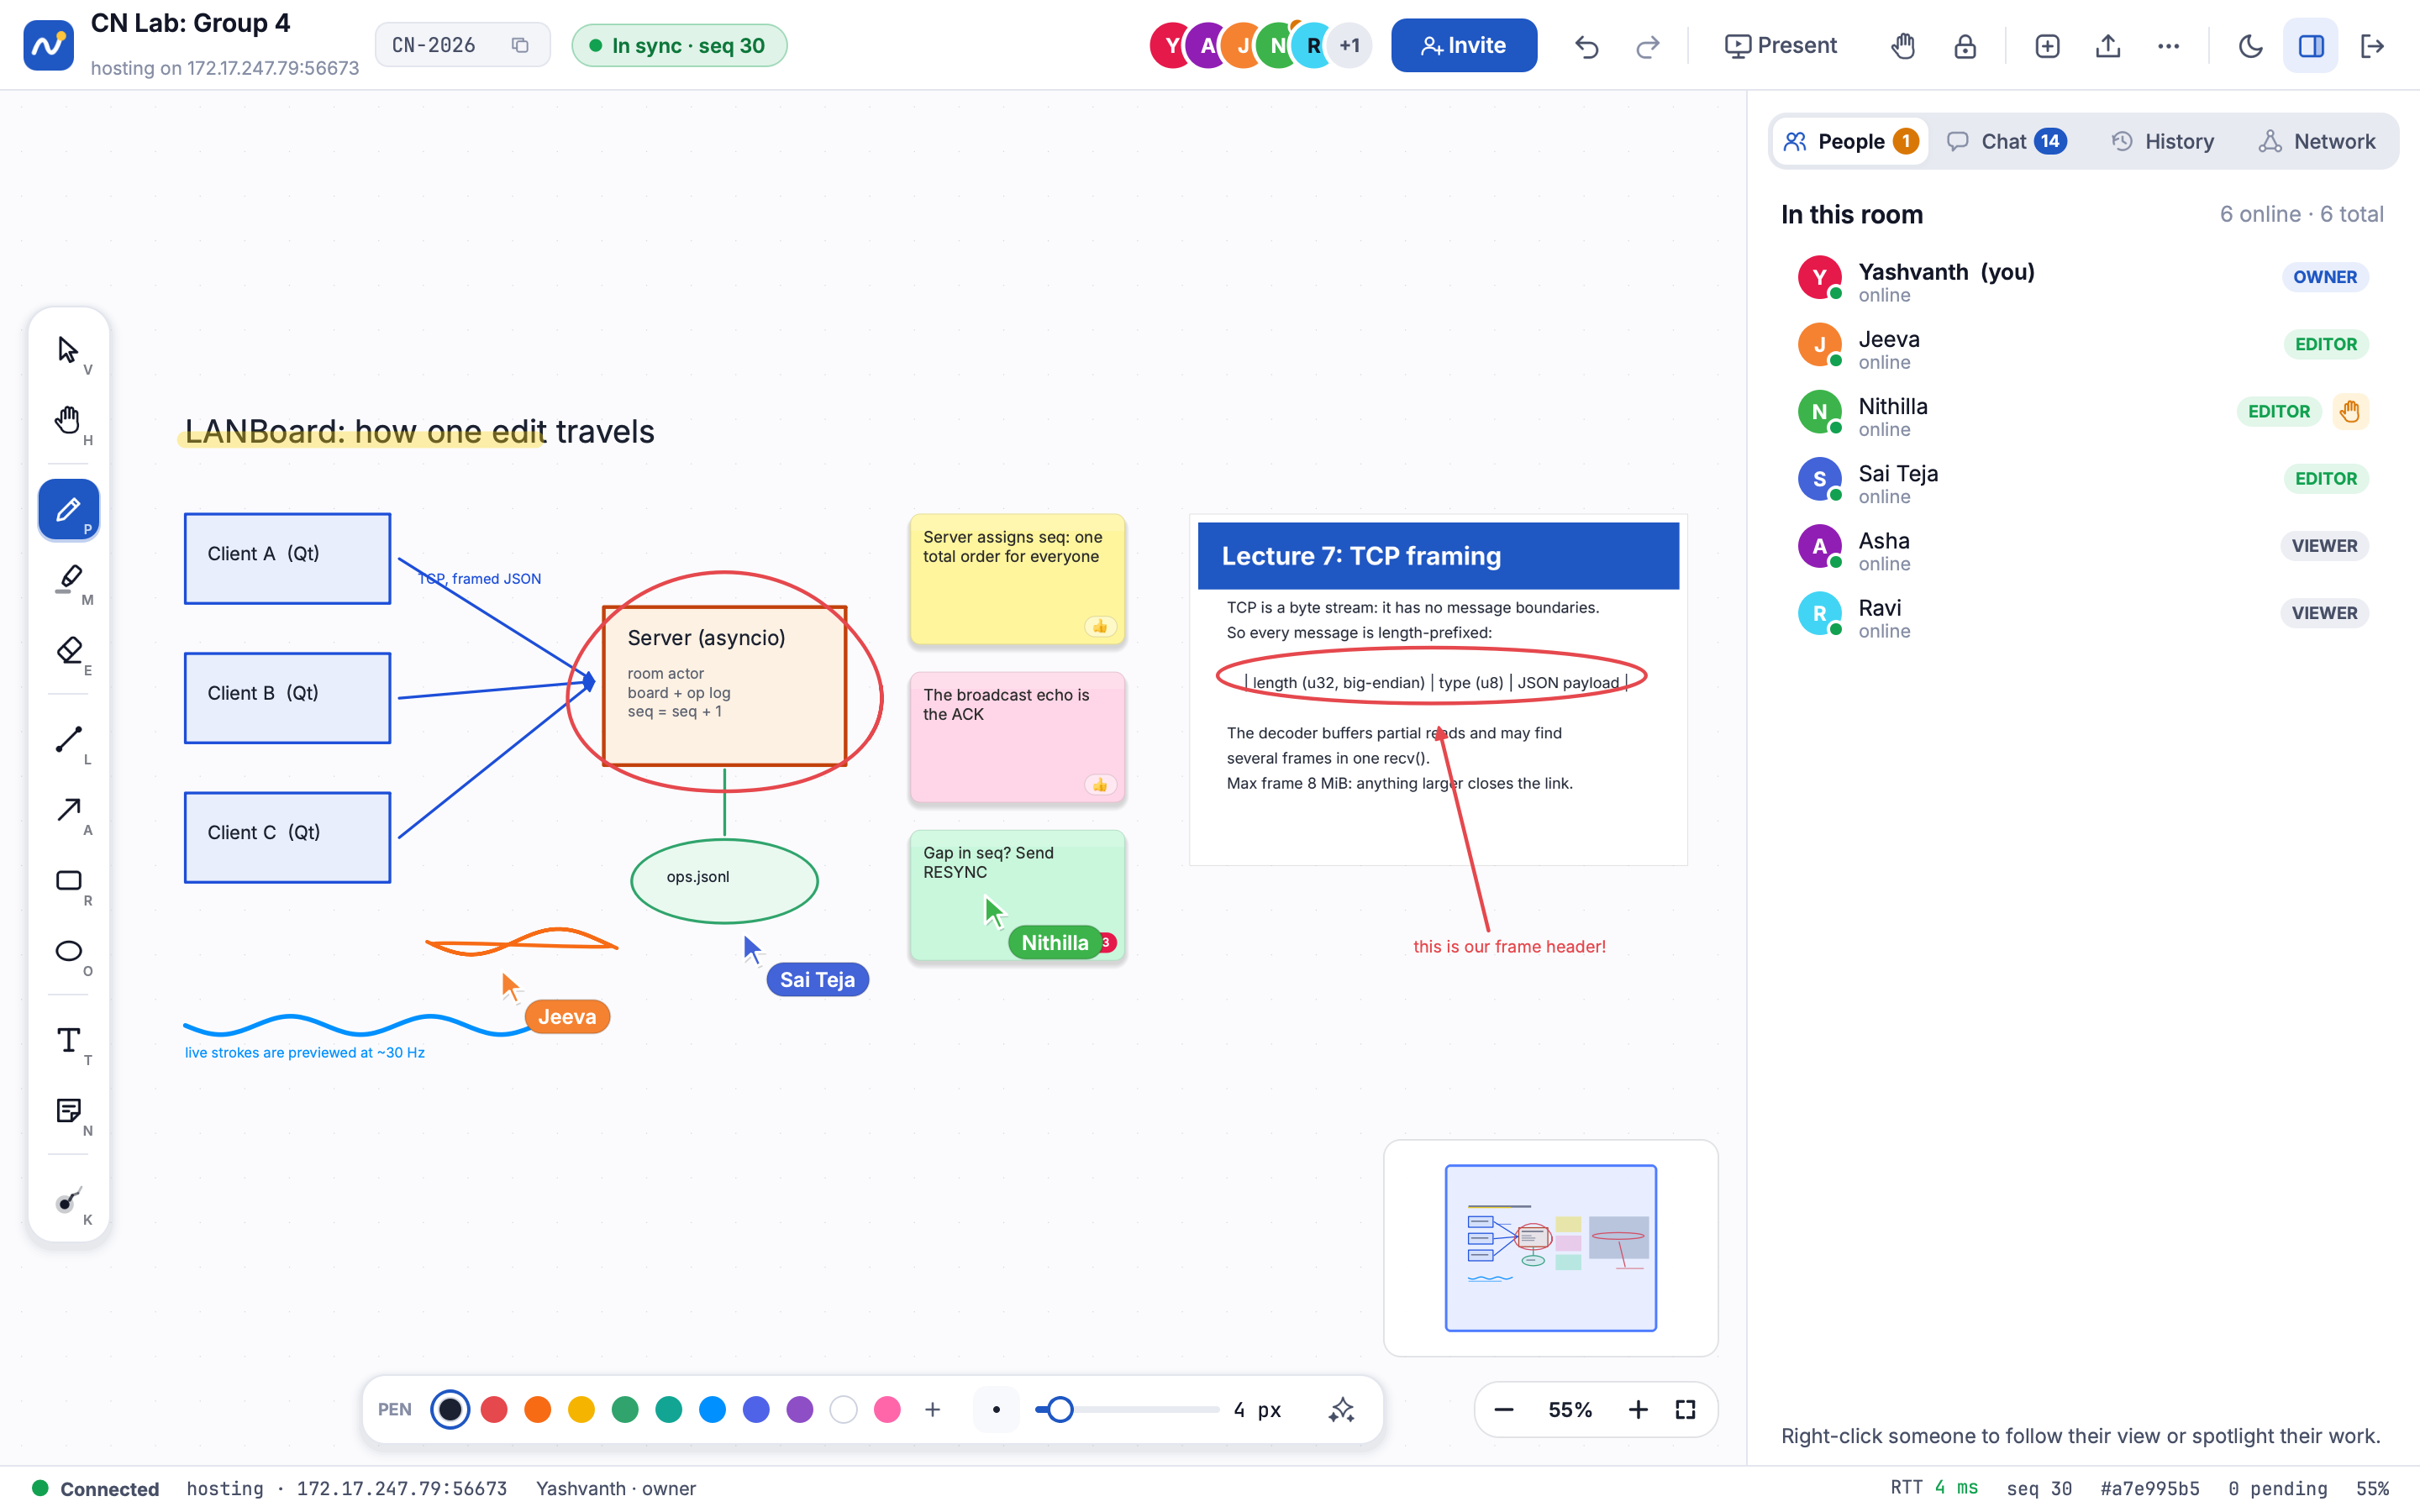
\includegraphics[width=0.82\textwidth]{../docs/assets/screens/light.png}
\caption{The client in the light theme, with several users drawing on one board.}
\end{figure}

\section{How it works}

Figure~\ref{fig:arch} shows the parts. Every edit (a stroke, a moved sticky note, a delete) is
sent to the server as an \emph{op}. The server checks it, gives it the next sequence number for
that room and sends it to every client in the room, including the one that sent it. Each client
applies ops strictly in sequence order, using the same \file{Board.apply} code as the server.
Since everyone starts from the same board and applies the same ops in the same order, everyone
ends up with the same board. This is the state machine idea from Schneider~\cite{schneider}, with
the server acting as the single sequencer that gives a total order in the sense of
Lamport~\cite{lamport}. Every 25 ops the server also sends a hash of its board, and a client whose
own hash differs asks for a fresh copy.

Board data goes over TCP port 5050. UDP port 5051 is used only for discovery, because only UDP
can broadcast. Short-lived things such as cursor positions and the preview of a stroke that is
still being drawn are relayed without a sequence number and are never stored.

\begin{figure}[h]
\centering
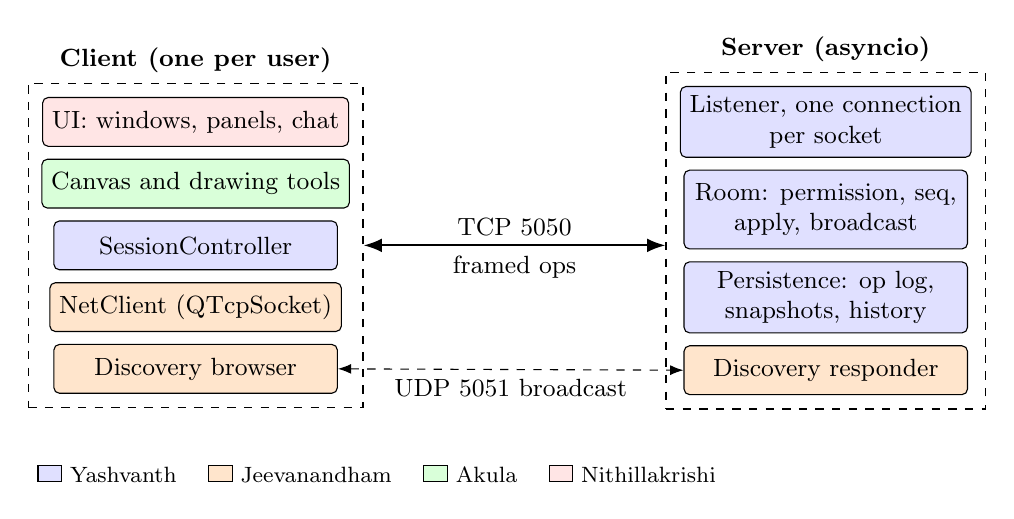
\begin{tikzpicture}[
  box/.style={draw, rounded corners=2pt, minimum width=3.6cm, minimum height=0.62cm,
              font=\small, align=center},
  mY/.style={box, fill=blue!12}, mJ/.style={box, fill=orange!20},
  mA/.style={box, fill=green!15}, mN/.style={box, fill=red!10},
  node distance=1.5mm]
  % client
  \node[mN] (ui) {UI: windows, panels, chat};
  \node[mA, below=of ui] (cv) {Canvas and drawing tools};
  \node[mY, below=of cv] (ctl) {SessionController};
  \node[mJ, below=of ctl] (net) {NetClient (QTcpSocket)};
  \node[mJ, below=of net] (disc) {Discovery browser};
  \node[draw, dashed, inner sep=5pt, fit=(ui)(disc),
        label={[font=\small\bfseries]above:Client (one per user)}] (client) {};
  % server
  \node[mY, right=4.2cm of ui] (lst) {Listener, one connection\\ per socket};
  \node[mY, below=of lst, minimum height=1.0cm] (room) {Room: permission, seq,\\ apply, broadcast};
  \node[mY, below=of room] (per) {Persistence: op log,\\ snapshots, history};
  \node[mJ, below=of per] (dresp) {Discovery responder};
  \node[draw, dashed, inner sep=5pt, fit=(lst)(dresp),
        label={[font=\small\bfseries]above:Server (asyncio)}] (server) {};
  % links
  \draw[{Latex}-{Latex}, thick] (client.east |- ctl) -- node[above, font=\small]{TCP 5050}
        node[below, font=\small]{framed ops} (server.west |- ctl);
  \draw[{Latex}-{Latex}, dashed] (disc.east) -- node[below, font=\small]{UDP 5051 broadcast}
        (dresp.west);
  % legend
  \node[below=6mm of client.south west, anchor=north west, font=\footnotesize] (leg) {%
    \tikz\fill[blue!12,draw=black] (0,0) rectangle (0.3,0.2); Yashvanth \quad
    \tikz\fill[orange!20,draw=black] (0,0) rectangle (0.3,0.2); Jeevanandham \quad
    \tikz\fill[green!15,draw=black] (0,0) rectangle (0.3,0.2); Akula \quad
    \tikz\fill[red!10,draw=black] (0,0) rectangle (0.3,0.2); Nithillakrishi};
\end{tikzpicture}
\caption{LANBoard parts, coloured by whose area they belong to. The controller is shared by
Yashvanth and Jeevanandham. The code in \file{common/} (framing, messages, board model) is used by
both sides.}
\label{fig:arch}
\end{figure}

\section{Yashvanth S: server core and state}

\textbf{Scope.} Yashvanth wrote the server, which lives in \file{server/}: \file{server.py},
\file{room.py}, \file{persistence.py} and the live terminal view in \file{dashboard.py}. He wrote
\file{common/model.py} together with Akula, and the part of \file{client/controller.py} that keeps
the confirmed copy of the board and applies ops in order. The headless bot in \file{tools/bot.py},
which we use for stress tests, is also his.

\textbf{How it works.} The whole server runs on one \texttt{asyncio} event loop~\cite{asyncio}.
Each socket gets a \file{ClientConnection} with a reader task and a writer task. The writer has a
queue that holds at most 4000 frames. If a client reads so slowly that its queue fills, the server
drops it as ``lagging'' instead of letting it slow down the whole room, and the client can resume
later. All room state is changed on that one thread, and \file{Room.submit} has no \texttt{await}
inside it, so there are no locks and no data races.

\file{Room.submit} handles one op in ten numbered steps. It checks that the sender has joined,
checks the role (a viewer cannot edit, a locked board blocks editors), applies a rate limit of 120
ops per second per client with a token bucket, validates the op, and drops an op whose
\texttt{op\_id} it has already accepted. It then normalises the op, rejects it if the frame would
be bigger than 4~MiB, gives it \texttt{seq = room.seq + 1}, applies it, writes it to disk and
broadcasts it. The copy that comes back to the sender is its acknowledgement.

Each accepted op is appended to \file{ops.jsonl} \emph{before} it is broadcast, which is the
write-ahead log idea~\cite{aries}. Every 50 ops or 10 seconds the server writes a snapshot of the
board: first to a temporary file, then \texttt{fsync}, then \texttt{os.replace}, so a crash never
leaves half a snapshot. Ops that leave the log move into \file{history.jsonl}, so the time-lapse
can still replay from the first op after a restart. Late joiners get the board as a
\texttt{SNAPSHOT}; a board above 1~MiB is cut into several frames tagged \texttt{part},
\texttt{parts} and \texttt{xid}, and the client applies it only when all parts have arrived.

\textbf{Problems and fixes.} The log is flushed after each line but not synced to disk, so a power
cut can leave a half-written last line. The loader skipped that torn line, but the next op was
appended straight onto it and was lost too. The fix was to end such a file with a newline before
appending. The second problem was harder to spot. If an op was accepted just before a client lost
its connection, and the resume was served with a full snapshot, the client never saw the echo for
that op. It stayed ``pending'' forever and was sent again on every reconnect. Now the server
answers the duplicate with the original op again, which settles it on the client. Both cases have
tests.

\section{Jeevanandham T: protocol and networking}

\textbf{Scope.} Jeevanandham wrote the wire format in \file{common/protocol.py} and the
message catalogue in \file{common/messages.py}. On the client he wrote \file{client/net.py} (the
\file{NetClient} with handshake, heartbeats and reconnect), \file{client/discovery.py}, the Chaos
Lab fault injector in \file{client/chaos.py} and the traffic counters in \file{client/metrics.py}.
His first commit put the shared \file{common/} package in place, so the rest of us had a fixed
wire format to code against from the first day.

\textbf{Framing.} TCP gives us a reliable, ordered stream of bytes~\cite{rfc793,rfc9293}, but it
does not keep message boundaries. One read can return half a message or five of them. So every
message is framed as a 4-byte big-endian length, then one type byte, then the payload as UTF-8
JSON. The length counts the type byte and the payload. \file{FrameDecoder.feed} adds whatever
bytes arrived to a buffer and then loops: if at least 4 bytes are there it reads the length; if
the whole frame is there it cuts it out and parses the JSON; otherwise it keeps the rest for the
next read. A length of 0, or more than 8~MiB, means the stream is broken, and the connection is
closed. The server and the client use the same decoder. The high half of the type byte groups the
messages: \texttt{0x0\_} control, \texttt{0x1\_} presence, \texttt{0x2\_} board ops,
\texttt{0x3\_} chat, and so on up to \texttt{0x6\_} for images. Both sockets set
\texttt{TCP\_NODELAY}, because Nagle's algorithm~\cite{rfc896} would hold back small cursor and
stroke frames.

\textbf{Discovery.} The client binds a UDP socket on any free port and sends a small datagram
\texttt{\{"magic": "LANBOARD\_DISCOVER\_V1"\}} to port 5051~\cite{rfc768}. It sends it to
\texttt{255.255.255.255}, to the directed broadcast address of every interface (such as
\texttt{192.168.1.255})~\cite{rfc919}, and to \texttt{127.0.0.1} for a server on the same
machine. Each server answers with a unicast reply containing its name, TCP port and rooms. The
reply does not contain the server's IP address; the client takes it from the sender address of
the datagram, which is an address it can actually reach. UDP may lose packets, so the client
probes every 2 seconds and forgets a server only after 6 seconds of silence.

\textbf{Heartbeat and reconnect.} The client sends a \texttt{PING} every 3 seconds with a
timestamp, and the server echoes it in a \texttt{PONG}, which gives the round-trip time without
synchronised clocks. A pulled cable sends no FIN or RST, so the connection just goes quiet. If
nothing arrives for 12 seconds, the side that is waiting declares the link dead. The client then
retries after 0.5, 1, 2 and 4 seconds and then every 5 seconds, each delay multiplied by a random
factor between 0.8 and 1.2 so that many clients do not all retry at the same instant. The new
\texttt{JOIN} carries a resume token and \texttt{last\_seq}, the last op the client applied. If
the server's log still has every op after \texttt{last\_seq}, and there are at most 5000 of them,
it sends just those in an \texttt{OP\_BATCH}; otherwise it sends a full snapshot. Ops the client
made while offline are sent again, and because each one has an \texttt{op\_id} of the form
\texttt{client\_id:counter}, the server never applies one twice. The same rules handle gaps
during normal use: an op with a sequence number that is too far ahead is held back, and if the
missing one has not arrived after 400~ms the client sends \texttt{RESYNC}. The Chaos Lab exists
because TCP hides loss on a healthy link. It drops, duplicates and delays incoming frames above
TCP, or cuts the connection, so that we can show these paths working live.

\textbf{Problems and fixes.} Before the demo we found two problems on real laptops. First, if port
5050 was already taken (often by an old server still running), the server crashed with a Python
traceback, and the client's Host mode would try to use whatever program was listening there.
Jeevanandham changed the server to print a clear message, suggest another port and exit with code
2. The client now sends a \texttt{PING} to the port first and reuses it only if a \texttt{PONG}
comes back. Second, on machines with more than one network adapter, the server printed the wrong
address or missed the real one, because it only looked at the interface behind the default
route. On a switch with the internet off there is no default route at all. He now lists the IPv4
address of every interface with the \texttt{SIOCGIFADDR} ioctl and sorts them so that normal LAN
ranges come first and VirtualBox, Docker and VPN addresses come last. The Invite box in the client
uses the same order.

\section{Akula Sai Teja: canvas and drawing}

\textbf{Scope.} Akula wrote the canvas in \file{client/canvas/}: \file{view.py} (pan,
zoom, image and PDF import, export), \file{scene.py}, \file{items.py}, \file{tools.py} and
\file{minimap.py}, plus \file{common/geometry.py}, the per-user undo in
\file{common/undo.py}, and \file{common/model.py} with Yashvanth. The builds are Akula's too:
the cross-platform PyInstaller spec~\cite{pyinstaller}, the smoke test, the GitHub Actions
workflow, the release zip script and the macOS app and DMG.

\textbf{How it works.} The canvas is a Qt \file{QGraphicsScene}~\cite{qt}, which gives us items,
hit testing, zoom and export to PNG, SVG and PDF. The rule is that tools never change the board
directly. They build an op and hand it to the controller, and the scene keeps one graphics item
per object id and rebuilds only the ids that changed. While you draw with the pen, the points go
out every 33~ms as a live preview that is never stored. When you lift the pen, the stroke is
simplified with the Ramer-Douglas-Peucker algorithm~\cite{ramer,douglas} at a tolerance of about
0.6 screen pixels, the numbers are rounded to one decimal place, and it is sent as one
\texttt{add} op. In our measurement a one-second stroke went from 121 points (1851 bytes) to 26
points (499 bytes). If you hold the pen still for 450~ms at the end, Smart Ink tries to recognise
a line, rectangle, ellipse or arrow and replaces the rough stroke with a clean shape.

Undo is per user. Your undo stack holds only your own ops, up to 500 of them, and an undo is sent
as a new inverse op, so the server orders it like any other edit. Before sending, the inverse is
filtered against the current board: for an update, only the properties that still have the value
you set are put back, so a later change by someone else is kept. If an object you added has
already been erased by another user, that undo entry is skipped. Images and PDF pages are stored
on the server as SHA-256 addressed blobs sent in 192~KiB chunks, and the op itself carries only
the hash.

\textbf{Problems and fixes.} The dark board made black ink nearly invisible. Changing the stored
colour would have broken the light-theme users and the exports, so Akula made the change
display-only: when painting on the dark board, very dark ink has its lightness mirrored and
near-white ink is mirrored the other way, while the op data and exports keep the real colour. The
same commit fixed a laser pointer head that could not be seen on white and resize handles that
viewers should not have seen. For the macOS app, the problem was Host mode. A frozen client
starts the server by looking for \file{lanboard-server} right next to its own executable, and a
plain \file{.app} bundle would have broken that. Akula put both executables into
\file{Contents/MacOS}, so the lookup still works, and added the local-network usage text that
newer macOS versions ask for before an app talks to other machines. The CI workflow builds and smoke-tests the
bundles on all three operating systems and also builds the DMG.

\section{Nithillakrishi P Y: user interface and collaboration}

\textbf{Scope.} Nithillakrishi built everything under \file{client/ui/}: the connect
dialog and server launcher, the main window, top bar and tool palette, the side panel with chat,
people and time-lapse history, the Network tab (HUD, Inspector and Chaos Lab panel), toasts,
dialogs and the light and dark theme. The later canvas-first redesign and the Windows
packaging fix are also Nithillakrishi's work.

\textbf{How it works.} The UI mirrors permissions but never enforces them. \file{\_update\_permissions}
greys out tools for a viewer or on a locked board, but the real check is on the server, so a
modified client still gets \texttt{FORBIDDEN}. The connect dialog fills ``Nearby servers'' from
the discovery browser, can generate a room code, and can start a server on the same computer. In
chat, the client sends the text, the server adds the id, time and sender, and broadcasts it, so
everyone sees the same order; a new joiner gets the recent messages in its \texttt{JOINED}
message. The time-lapse replays history into a separate board, so the live board keeps syncing
underneath, and the owner can restore an old version for everyone. The Network Inspector lists
every frame this client sends or receives, with its direction, type, size, sequence number, chaos
tag and decoded JSON. The sync badge in the top bar is green only when the last board hash from
the server matched our own. Fonts (Inter and JetBrains Mono) are bundled and icons are drawn in
code, so nothing is fetched from the internet.

\textbf{Problems and fixes.} The Windows executable built with Python 3.14 would not start.
PyInstaller had collected an \file{icuuc.dll} whose exports did not match what Qt expected.
Nithillakrishi changed \file{packaging/lanboard.spec} to leave that DLL out of both bundles on
Windows, so Qt uses the system one. In the UI, the Network tab clipped its labels when the side
panel was 360 to 400 pixels wide. The fix was eliding, shorter byte units and fixed-width columns.
The sync badge also claimed things it did not know yet, so it now shows ``Connecting'' or
``Signing in'' before the first join and says ``edits queued'' only when there really are queued
edits. The redesign commit also fixed theme-change handlers that were still being called
after their widgets had been deleted.

\section{How we worked together}

We split the work by layer and agreed on the wire format and the module contracts
(\file{docs/CLIENT\_API.md}) first, so each of us could work and test alone. Jeevanandham's
\file{common/} package went in first, then the server, the controller, the network client, the
canvas and the UI. Each member committed their own area from their own account, and the git
history shows who did what.

Yashvanth did most of the integration. He wrote the controller that connects the network client
to the canvas, wrote the end-to-end tests that run everything together, and fixed problems that
showed up between modules, such as Qt crashes when a socket was torn down during a reconnect and
offline edits being replayed faster than the server's rate limit allowed. He also helped
Jeevanandham and Nithillakrishi directly and worked with them on several of their commits. He
wrote most of the documentation and checked the numbers in it against the code.

\section{Testing}

The suite has 318 tests and they all pass in about 95 seconds (\texttt{.venv/bin/python -m pytest
-q}). Most of them are unit tests: 13 for framing, 40 for the board model, 44 for the server's
room logic, 27 for the network client, 17 for the controller, 32 for the canvas and 28 for
geometry. Thirty integration tests run the real server and bot clients over real sockets,
including passwords, kicks, timeouts, a slow reader being dropped, resume and crash recovery.

The convergence test lets six bots edit one board for 3 seconds at 40 ops per second each, while
they randomly disconnect, keep editing offline and resume. At the end every bot's board hash must
equal the server's. A second run shrinks the server history to 8 ops, so most resumes need a full
snapshot instead of a replay. In \file{test\_e2e\_client.py}, real Qt clients run against a real
server; one test turns on the Chaos Lab with 30\% drops, 30\% duplicates and 20 to 60~ms of
delay, and the board still converges. \file{test\_e2e\_app.py} goes further: 39 tests open two or
three complete windows and drive them with real mouse and keyboard events, then check that the
other window sees the result. Writing those tests found nine bugs, which are fixed. On top of
this, CI runs the frozen executables on Windows, Linux and macOS, where four bots must converge,
and an 8-bot stress run on loopback handled 1771 ops in about 12 seconds with no resyncs.

\begin{thebibliography}{99}
\setlength{\itemsep}{1pt}
\small

\bibitem{rfc793} J.~Postel. \emph{Transmission Control Protocol}. RFC 793, IETF, September 1981.

\bibitem{rfc9293} W.~Eddy (Ed.). \emph{Transmission Control Protocol (TCP)}. RFC 9293, IETF,
August 2022.

\bibitem{rfc896} J.~Nagle. \emph{Congestion Control in IP/TCP Internetworks}. RFC 896, IETF,
January 1984.

\bibitem{rfc768} J.~Postel. \emph{User Datagram Protocol}. RFC 768, IETF, August 1980.

\bibitem{rfc919} J.~Mogul. \emph{Broadcasting Internet Datagrams}. RFC 919, IETF, October 1984.

\bibitem{lamport} L.~Lamport. Time, clocks, and the ordering of events in a distributed system.
\emph{Communications of the ACM}, 21(7):558--565, 1978.

\bibitem{schneider} F.~B.~Schneider. Implementing fault-tolerant services using the state machine
approach: a tutorial. \emph{ACM Computing Surveys}, 22(4):299--319, 1990.

\bibitem{aries} C.~Mohan, D.~Haderle, B.~Lindsay, H.~Pirahesh and P.~Schwarz. ARIES: a
transaction recovery method supporting fine-granularity locking and partial rollbacks using
write-ahead logging. \emph{ACM Transactions on Database Systems}, 17(1):94--162, 1992.

\bibitem{ramer} U.~Ramer. An iterative procedure for the polygonal approximation of plane curves.
\emph{Computer Graphics and Image Processing}, 1(3):244--256, 1972.

\bibitem{douglas} D.~H.~Douglas and T.~K.~Peucker. Algorithms for the reduction of the number of
points required to represent a digitized line or its caricature. \emph{The Canadian
Cartographer}, 10(2):112--122, 1973.

\bibitem{asyncio} Python Software Foundation. \emph{asyncio: Asynchronous I/O}. Python 3
documentation, \url{https://docs.python.org/3/library/asyncio.html}.

\bibitem{qt} The Qt Company. \emph{Qt for Python (PySide6) documentation}: QTcpSocket,
QUdpSocket and the Graphics View Framework. \url{https://doc.qt.io/qtforpython-6/}.

\bibitem{pyinstaller} PyInstaller Development Team. \emph{PyInstaller Manual}.
\url{https://pyinstaller.org/}.

\end{thebibliography}

\end{document}
